\chapter {Design of OGM library}

We should now have all information we need to propose our solution for OGM using the C\# language.
Before we start to analyze individual pieces of the library needed for its proper function, we need a list of requirements.

The solution should be able to:
\begin{itemize}
    \item {connect to a database}
    \item {map objects into graph structure}
    \item {map LINQ query into Cypher query}
    \item {execute a command in a database}
    \item {retrieve a result from the database}
    \item {map the result from the database into objects}
\end{itemize}

With these minimal requirements set, we can now go through them, analyze them, and propose individual solutions to them.

\section{Connect to a database}

Neo4j company has created a client for .NET that supports both bolt and neo4j URI schemes. \cite{noauthor_client_nodate} This driver is a standalone NuGet package that is publicly accessible and licensed under Apache 2.0 license. This means we can use this driver in our library as a dependency.

The application should handle the driver's lifecycle. During startup, the application should create an instance of the driver and then correctly destroy this instance on exit. The lifecycle will be managed by our library or by using DIC.

Before we create an instance of the driver, we need to pass the correct configuration for the driver. Configuration for the driver and session must be created and maintained. .NET does contain a configuration manager used with the linkage to dependency injection.

Here is visualisation of connections between components:

\begin{figure}[H]
    \centering
    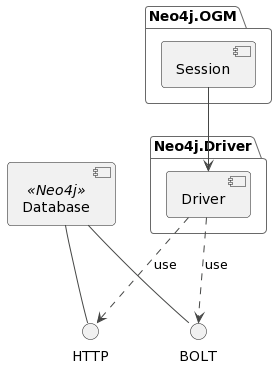
\includegraphics[width=0.4\textwidth]{content/components.png}
    \caption{Components diagram}
\end{figure}

\subsection{Conclusion}

We will use Neo4j's official driver for connection, but we need to encapsulate it into our library.
We need to create a configuration structure and configuration builder, which will then be used to create a connection to the database.

\section {Map objects into graph structure}

If we want to correctly translate queries from the object paradigm into Cypher, we need to know the graph structure described in our domain.

What we are trying to do is create metadata. To build metadata, we first need information, which assemblies contain models representing nodes and relationships in a graph. A developer must declare these assemblies as it is necessary to limit the scope that will be scanned using reflection.

The solutions we analyzed in the previous chapter are internally working very similarly. Both are scanning assemblies or packages on initialization (Java uses packages vs. C\# uses assemblies/namespaces), and we will borrow some of the features from these solutions into ours.
Developers of our library will need to define a set of assemblies. During the initialization of our library, we will scan these assemblies and create a metadata object with information about the user-defined graph.

\subsection {Annotations}

To create a metadata object, we need to identify and process nodes and relationships. We need to have a way for developers to describe each node and its relationship with all properties they would want to define, and which we also need to build the metadata object correctly.

We already have a solution to this problem, and Neo4j also uses it to solve the same issue. We will use annotations using attributes. Using these annotations, we can describe nodes and their relationships.

We will look for these annotations during initialization using reflection, which is well supported by C\# and .NET. With annotation, we can describe the graph and create the metadata object.

\subsection {Entity mapper}

Entity mapper should be able to map entities into statements that could then be translated into Cypher query. It should be able to use generated metadata correctly
to map both nodes and relationships.

For this purpose, we will define a interface \texttt{IEntityMapper}. This interface will contain
this list of public methods:

\begin{itemize}
    \item {\texttt{Map}: this method map an entity to a \texttt{ICompilerContext}}
    \item {\texttt{CompilerContext}: this method returns a current instance of\linebreak\texttt{ICompilerContext}}
\end{itemize}

In the picture \ref{fig:IEntityMapperClassDiagram} is class diagram with interfaces and also classes that implements these interfaces.
The interface \texttt{ICompilerContext} contains methods for controlling the context of mapped nodes and relationships. These methods
are used during mapping an entity in \texttt{IEntityMapper.Map} method to map an entity for Cypher query.

\begin{figure}[H]
    \centering
    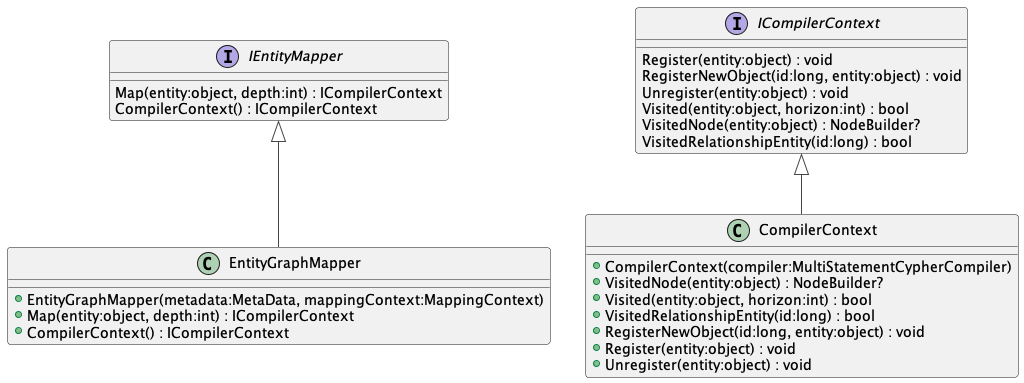
\includegraphics[width=0.8\textwidth]{content/entitymapper.png}
    \caption{\texttt{IEntityMapper} and \texttt{ICompilerContext} class diagrams}
    \label{fig:IEntityMapperClassDiagram}
\end{figure}

\section {Map LINQ query into Cypher query}

Mapping a LINQ query to a Cypher query is a bit more complicated. As we already know, any LINQ query is an expression tree used to process an IQueryable object.
We cannot map these expressions to a Cypher query because we do not know how to map the expression tree to a Cypher query. However, there is a way to transform the expression tree
into a Cypher query. We know this because Entity Framework does the same thing for SQL queries. We can illustrate the process of transformation using the state diagram
\ref{fig:querystate}.

\begin{figure}[H]
    \centering
    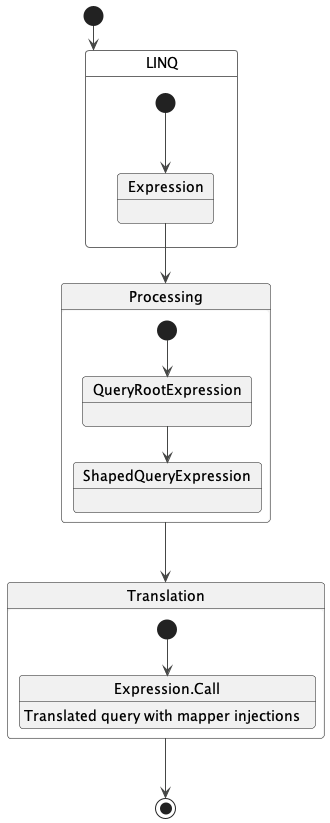
\includegraphics[width=0.5\textwidth]{content/Expression transformation.png}
    \caption{LINQ expression transformation}
    \label{fig:querystate}
\end{figure}

\subsection{\texttt{IQueryable} extension}

If we want to communicate with the database, the \texttt{IQueryable} instance must have a correct provider.
This provider must be able to transform the expression tree into a Cypher query and also execute the query asynchronously. We are going to extend \texttt{IQueryProvider} interface
with \texttt{IAsyncQueryProvider} interface which declares \texttt{IAsyncQueryProvider.ExecuteAsync<T>} method.

To set a correct provider we are going to define new class that implements \texttt{IQueryable<T>} interface called \texttt{DbSet<T>}.
The name of the class is the same as it is in Entity Framework. Besides implementing \texttt{IQueryable<T>} interface \texttt{DbSet<T>} class also implements
\texttt{IAsyncEnumerable<T>} interface. This interface is used to create an asynchronous enumerable object.

Inside the constructor of \texttt{DbSet<T>} class, we are going to set the correct provider as well as set an instance of \texttt{ISession}.
Because we need an instance of \texttt{ISession} we are going to declare a method inside this interface called
\texttt{ISession.Set<TEntity>} which will create a new instance
of \texttt{DbSet<T>}.

Because we are communicating with a database using asynchronous operations, we need to create extension methods for \texttt{DbSet<T>} which are also asynchronous.
For example, LINQ has method called \texttt{FirstOrDefault} which returns first element of \texttt{IQueryable<T>} or default value of type T. We are going to create
an extension of \texttt{IQueryable<T>} with method \texttt{FirstOrDefaultAsync}. This extension method will transform the expression tree into a Cypher query.

Inside this extension method, we will call providers\linebreak
\code{IAsyncQueryProvider.ExecuteAsync<T>} method. This is our entry point, from which we will start a translation
of the expression tree into a Cypher query.

For better visualisation, here \ref{fig:queryprovider} is class diagram of query provider and\linebreak\texttt{DbSet<T>} class.

\begin{figure}[H]
    \centering
    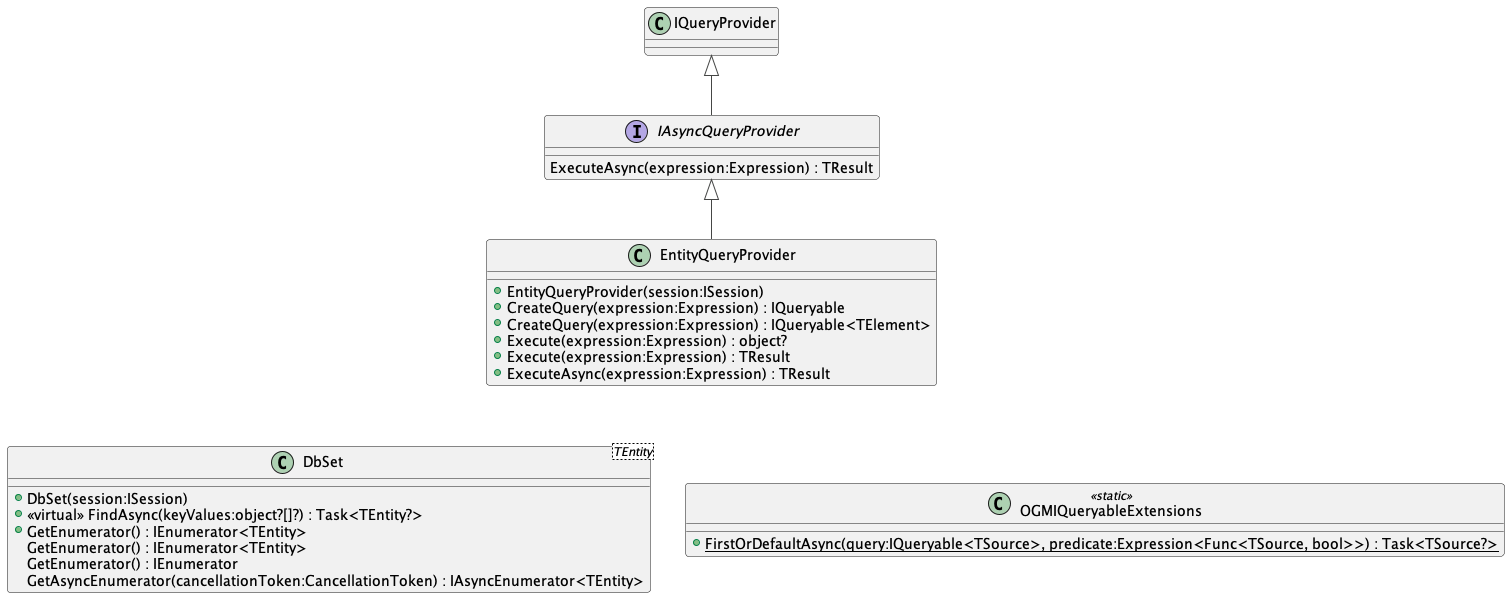
\includegraphics[width=0.9\textwidth]{content/QueryProvider.png}
    \caption{\texttt{IAsyncQueryProvider} and \texttt{DbSet<TEnity>} with extension class diagram}
    \label{fig:queryprovider}
\end{figure}

\subsection{Query compilation}

To best visualize the process of query compilation, we will use sequence
diagram \ref{fig:QueryCompilerSequence}. In this diagram, we can see how we will employ
the\linebreak\texttt{ExpressionVisitor} abstract class to visit the expression tree and, through the different steps, recreate it to the state which is needed to compile the Cypher query.

The result of this compilation will be a \texttt{Func<QueryContext, TResult>}, which is an object representing the function.
This function does both a query execution and enumerates a result from a database response.

In the sequence diagram \ref{fig:QueryCompilerSequence}, are three expression tree visitors, each serving different purpose. Using these visitors
gives us the ability to expand our library's capabilities easily. We would only need to create a new visitor who would comply with
the existing expression. We can also further expand the capabilities of defined visitors inside their implementation.

We should also introduce the concerns of each visitor. The first one that is used in the diagram is \texttt{ParameterExtractingExpressionVisitor},
which extracts parameters from the original expression. The next one is\linebreak\texttt{QueryableMethodTranslationExpressionVisitor}, this visitor will
be responsible for translating the original LINQ query into an expression tree that will be consisted of \texttt{CypherExpression} derivatives,
which will copy the Cypher language structure. The last visitor is\linebreak\texttt{ShapedQueryCompilinExpressionVisitor}, it is responsible
for taking a\linebreak\texttt{ShapedQueryExpression} and translating it into a \texttt{Expression.Call} expression, which can be then compiled into
the \texttt{Func<QueryContext, TResult>} object.

\begin{figure}[H]
    \centering
    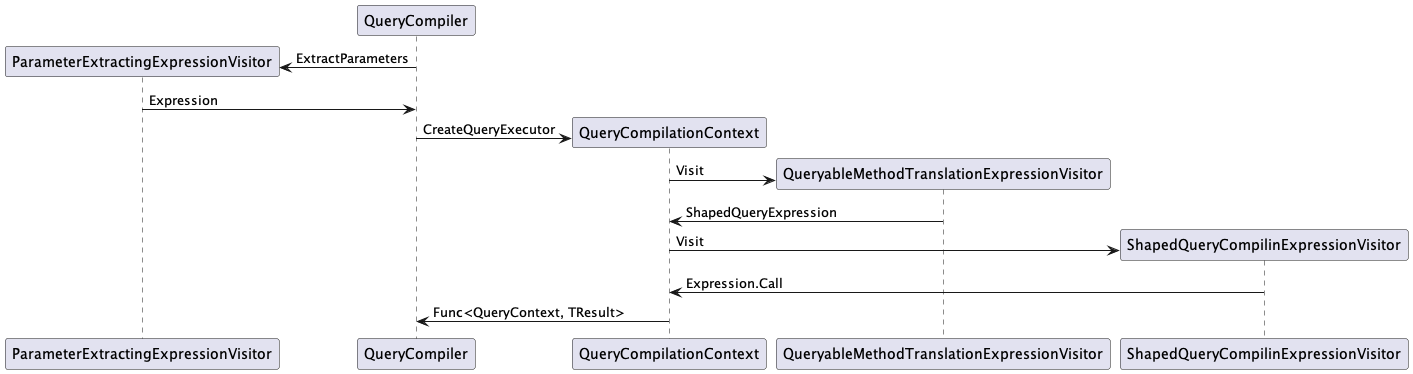
\includegraphics[width=\textheight, angle=90]{content/Translation Sequence.png}
    \caption{\texttt{QueryCompiler} compilation sequence}
    \label{fig:QueryCompilerSequence}
\end{figure}

\section{Execute a command and retrieve the result}

We will be using Neo4js official driver for .NET to execute the query. The result of any query
is returned using \texttt{IResultCursor} interface. This interface is somewhat similar to an asynchronous
enumerator, but it does not implement the \texttt{IAsyncEnumerable<T>} interface. The \texttt{IResultCursor} interface
declares methods as show on the \ref{fig:iresinterface} picture. We will have to adapt our code to use this interface.
We are going to use these methods inside a proper implementation of \texttt{IAsyncEnumerable<T>}
interface.

\begin{figure}[H]
    \centering
    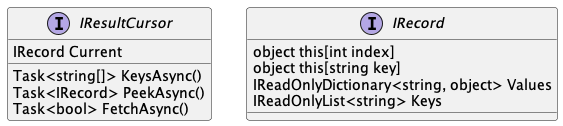
\includegraphics[width=0.7\textwidth]{content/IResultCursor.png}
    \caption{\texttt{IResultCursor} and \texttt{IRecord} interfaces}
    \label{fig:iresinterface}
\end{figure}

\section{Map the result of the query to an object}

Mapping result into an object is our last step. We already know from \ref{fig:iresinterface} class diagram,
that we can access an \texttt{IRecord} interface using \texttt{IResultCursor.Current} property.
This interface represents a single result of the query, which is defined in Cypher using \texttt{RETURN} clause.

Our mapper needs to read the result and correctly choose the right key from the values. IRecord is not a representation of a single node or relationship, but it is a representation of the \texttt{RETURN} clause, meaning that it contains all the values of the \texttt{RETURN} clause.
Mapper needs to know which key contains which entity and or value.

We can solve this issue by creating an extension method that will extend an \texttt{IRecord} interface and accept a \texttt{string} parameter defining an alias of value.
This method will return either a value or an entity.

\section{Summary}

In this chapter, we designed a solution for an \acrshort{ogm} library in .NET with LINQ to Cypher translation.
We started with defining six critical requirements that our library must solve and then went through each one of them and
proposed a solution for them.

We defined how we would handle creating a connection to the database using Neo4js official driver for .NET. Then we moved on
to the problem of mapping objects into graph structure using annotations and reflection. We also proposed a solution for mapping LINQ queries to
Cypher queries. At the end of this chapter, we went through the process of executing and mapping the Cypher query and its result back into objects.

With this design, we should have all that we need to successfully implement \acrshort{ogm} library for .NET with LINQ to Cypher translation.

\todo[inline]{create diagram for expression tree changes}